\ifdefined\beamerclass
\else
    \def\beamerclass{beamer}
\fi
\documentclass[\beamerclass]{beamer}

\usepackage{pgfpages}
\mode<handout>{
	% \setbeamercolor{background canvas}{bg=black!20}
	\pgfpagesuselayout{2 on 1}[a4paper,border shrink=5mm]
}

\usepackage{lmodern}
\usepackage{listings}
\usepackage{amsmath}
\usepackage{bm}
\usepackage{textpos} % package for the positioning

\usepackage{pgf, tikz}
\usetikzlibrary{arrows, automata}

\usetheme{Copenhagen}
\hypersetup{pdfstartview={Fit}}
\lstset{basicstyle=\small\ttfamily,breaklines=true}

\title[Automatic Differentiation]{An Introduction to Automatic Differentiation}
\author{Jonathon Hare}
\institute[]
{
  Vision, Learning and Control\\
  University of Southampton 
}
\date{}
\subject{Computer Science}
\useoutertheme{infolines}
\setbeamertemplate{headline}{} %remove headline
\setbeamertemplate{navigation symbols}{} %remove navigation symbols

\definecolor{darkblue}{RGB}{37,55,97}
\definecolor{mellowyellow}{RGB}{247,206,70}
\definecolor{almostwhite}{RGB}{254,255,255}
\definecolor{merrygreen}{RGB}{79,173,91}
\definecolor{funkyorange}{RGB}{240,154,56}

\addtobeamertemplate{footnote}{\hskip -2em}{}
\newcommand\blfootnote[1]{%
  \begingroup
  \renewcommand\thefootnote{}\footnote{#1}%
  \addtocounter{footnote}{-1}%
  \endgroup
}

\begin{document}

\begin{frame}[plain]
        \begin{tikzpicture}[overlay, remember picture, shift={(current page.south west)},font={\fontfamily{Montserrat-TOsF}\selectfont}]
        \fill [merrygreen,text=darkblue] (0,0) rectangle (\paperwidth, \paperheight);
        \draw (4,7) node [align=left,text=almostwhite] {\Huge \begin{tabular}{l} \textbf{Differentiate} \\ \textbf{Automatically} \end{tabular}};
        \draw (11,1) node [align=left,text=almostwhite] {\includegraphics[scale=0.15]{../vlc.png}};
        \end{tikzpicture}
\end{frame}

  \frame{
  \titlepage

\tiny{Much of this material is based on this blog post:
\url{https://rufflewind.com/2016-12-30/reverse-mode-automatic-differentiation}}
  }

\begin{frame}
\frametitle{What is Automatic Differentiation (AD)?}
To solve optimisation problems using gradient methods we need to compute the gradients (derivatives) of the objective with respect to the parameters.
\begin{itemize}
	\item In neural nets we're talking about the gradients of the loss function, $\mathcal{L}$ with respect to the parameters $\bm{\theta}$: 
	$\nabla_{\bm{\theta}} \mathcal{L} = \frac{\partial \mathcal{L}}{\partial \bm{\theta}}$
	\item AD is important - it's been suggested that ``Differentiable programming'' could be the term that ultimately replaces deep learning\footnote{\url{http://forums.fast.ai/t/differentiable-programming-is-this-why-we-switched-to-pytorch/9589/5}}.
\end{itemize}
\end{frame}

\begin{frame}
	\frametitle{What is Automatic Differentiation (AD)?}
	\framesubtitle{Computing Derivatives}
There are three ways to compute derivatives:

\begin{columns}
	\column{.45\textwidth}
    \setbeamercovered{transparent}
    \begin{itemize}
    	\item<1,2> Symbolically differentiate the function with respect to its parameters
    	\begin{itemize}
    		\item by hand
    		\item using a CAS
    	\end{itemize}
    	\item<1,3> Make estimates using finite differences
    	\item<1,4> Use Automatic Differentiation
    \end{itemize}

    \column{.45\textwidth}
      \begin{block}{Problems}<2>
        Static - can't ``differentiate algorithms''
      \end{block}
      \begin{block}{Problems}<3>
        Numerical errors - will compound in deep nets
      \end{block}
  \end{columns}
\end{frame}

\begin{frame}
	\frametitle{What is Automatic Differentiation (AD)?}

	Automatic Differentiation is:
	\begin{itemize}
		\item a method to get exact derivatives efficiently, by storing information as you go forward that you can reuse as you go backwards.
		\begin{itemize}
			\item Takes code that computes a function and uses that to compute the derivative of that function.
		\item The goal isn't to obtain closed-form solutions, but to be able to write a program that efficiently computes the derivatives.
		\end{itemize}
	\end{itemize}
\end{frame}

\begin{frame}[fragile]
\frametitle{Lets think about differentiation and programming}
\begin{columns}
	\column{.45\textwidth}
    \begin{example}<1->[Math] 
    \vspace{-1.5em}
    \begin{align*}
			x & = ? \\
			y & = ? \\
			a & = x \, y \\
			b & = \sin(x) \\
			z & = a + b
		\end{align*}
    \end{example}

	\column{.45\textwidth}
	\begin{example}<2->[Code]
			\begin{lstlisting}
x = ?
y = ?
a = x * y
b = sin(x)
z = a + b
			\end{lstlisting}
	\end{example}
	\end{columns}
\end{frame}

\begin{frame}
\frametitle{The Chain Rule of Differentiation}

\uncover<1->{
Recall the chain rule for a variable/function $z$ that depends on $y$ which depends on $x$:
\begin{equation*}
\frac{dz}{dx} = \frac{dz}{dy}\frac{dy}{dx}
\end{equation*}
}

\uncover<2->{
In general, the chain rule can be expressed as:
\begin{equation*}
	\frac{\partial w}{\partial t} = \sum_i^N \frac{\partial w}{\partial u_i} \frac{\partial u_i}{\partial t} = \frac{\partial w}{\partial u_1}\frac{\partial u_1}{\partial t} + \frac{\partial w}{\partial u_2}\frac{\partial u_2}{\partial t} + \dots + \frac{\partial w}{\partial u_N}\frac{\partial u_N}{\partial t}
\end{equation*}
where $w$ is some output variable, and $u_i$ denotes each input variable $w$ depends on.
}
\end{frame}

\begin{frame}
\frametitle{Applying the Chain Rule}

Let's differentiate our previous expression with respect to some yet to be given variable $t$:
\begin{columns}
\column{.3\textwidth}
\begin{block}<1->{Expression}
    \vspace{-1.5em}
    \begin{align*}
			x & = ? \\
			y & = ? \\
			a & = x \, y \\
			b & = \sin(x) \\
			z & = a + b
		\end{align*}
    \end{block}

\column{.65\textwidth}
\begin{align*}
	\frac{\partial x}{\partial t} & = ? \\
	\frac{\partial y}{\partial t} & = ? \\
	\frac{\partial a}{\partial t} & = x \frac{\partial y}{\partial t} + y \frac{\partial x}{\partial t}\\
	\frac{\partial b}{\partial t} & = \cos(x) \frac{\partial x}{\partial t}\\
	\frac{\partial z}{\partial t} & = \frac{\partial a}{\partial t} + \frac{\partial b}{\partial t}
\end{align*}
\end{columns}
\vfill
 
\uncover<2->{If we substitute $t=x$ in the above we'll have an algorithm for computing $\partial z/\partial x$. To get $\partial z/\partial y$ we'd just substitute $t=y$.
}

\end{frame}

\begin{frame}[fragile]
\frametitle{Translating to code I}
We could translate the previous expressions back into a program involving \emph{differential variables} \lstinline!{dx, dy, ...}! which represent $\partial x/\partial t, \partial y/\partial t, \dots$ respectively:

\begin{lstlisting}
dx = ?
dy = ?
da = y * dx + x * dy
db = cos(x) * dx
dz = da + db	
\end{lstlisting}

\uncover<2->{What happens to this program if we substitute $t=x$ into the math expression?}
\end{frame}

\begin{frame}[fragile]
\frametitle{Translating to code II}

\begin{columns}
\column{.45\textwidth}
\begin{lstlisting}
dx = 1
dy = 0
da = y * dx + x * dy
db = cos(x) * dx
dz = da + db	
\end{lstlisting}

\column{.45\textwidth}

\uncover<2->{The effect is remarkably simple: to compute $\partial z/\partial x$ we just seed the algorithm with \lstinline!dx=1! and \lstinline!dy=0!.}
\end{columns}
\end{frame}


\begin{frame}[fragile]
\frametitle{Translating to code III}

\begin{columns}
\column{.45\textwidth}
\begin{lstlisting}
dx = 0
dy = 1
da = y * dx + x * dy
db = cos(x) * dx
dz = da + db	
\end{lstlisting}

\column{.45\textwidth}

To compute $\partial z/\partial y$ we just seed the algorithm with \lstinline!dx=0! and \lstinline!dy=1!.
\end{columns}
\end{frame}

\begin{frame}[fragile]
\frametitle{Making Rules}

\begin{itemize}
	\item<+-> We've successfully computed the gradients for a specific function, but the process was far from automatic. 
	\item<+-> We need to formalise a set of rules for translating a program that evaluates an expression into a program that evaluates its derivatives.
	\item<+-> We have actually already discovered 3 of these rules:
\begin{lstlisting}
c = a + b   =>  dc = da + db
c = a * b   =>  dc = b * da + a * db
c = sin(a)  =>  dc = cos(a) * da
\end{lstlisting}
\end{itemize}

\end{frame}

\begin{frame}[fragile]
\frametitle{More rules}

These initial rules:
\begin{lstlisting}
c=a+b     =>  dc=da+db
c=a*b     =>  dc=b*da+a*db
c=sin(a)  =>  dc=cos(a)*da
\end{lstlisting}
can easily be extended further using multivariable calculus:
\begin{lstlisting}
c=a-b     =>  dc=da-db
c=a/b     =>  dc=da/b-a*db/b**2
c=a**b    =>  dc=b*a**(b-1)*da+log(a)*a**b*db
c=cos(a)  =>  dc=-sin(a)*da
c=tan(a)  =>  dc=da/cos(a)**2
\end{lstlisting}
\end{frame}

\begin{frame}
\frametitle{Forward Mode AD}
\begin{itemize}
	\item<+-> To translate using the rules we simply replace each primitive operation in the original program by its differential analogue.
	\item<+-> The order of computation remains unchanged: if a statement $K$ is evaluated before another statement $L$, then the differential analogue of $K$ is evaluated before the analogue statement of $L$.
	\item<+-> This is \textbf{Forward-mode Automatic Differentiation}.
\end{itemize}
\end{frame}

\begin{frame}[fragile]
\frametitle{Interleaving differential computation}

A careful analysis of our original program and its differential analogue shows that its possible to interleave the differential calculations with the original ones:
\begin{columns}
	\column{.45\textwidth}
\begin{lstlisting}
x  = ?
dx = ?

y  = ?
dy = ?

a  = x * y
da = y * dx + x * dy

b  = sin(x)
db = cos(x) * dx

z  = a + b
dz = da + db
\end{lstlisting}

\column{.45\textwidth}
\begin{block}{Dual Numbers}<2->
	\begin{itemize}
		\item<2-> This implies that we can keep track of the value and gradient at the same time.
		\item<3-> We can use a mathematical concept called a ``Dual Number'' to create a very simple direct implementation of AD.
	\end{itemize}
\end{block}

\end{columns}
\end{frame}

% \begin{frame}
% \frametitle{Forward Mode AD}
% \begin{block}{Let's try this for ourselves\ldots}
% \begin{itemize}
% 	\item Clone the git repository: \lstinline!git clone git@github.com:ecs-vlc/understanding-autograd.git!
% 	\item Launch \lstinline!jupyter notebook! and load the \lstinline!ForwardAD.ipynb! notebook.
% 	\item Work through the exercises.
% \end{itemize}
% \end{block}
% \end{frame}

\begin{frame}
\frametitle{Reverse Mode AD}
\begin{itemize}
	\item<+-> Whilst Forward-mode AD is easy to implement, it comes with a very big disadvantage\ldots
	\item<+-> \textbf{For every variable we wish to compute the gradient with respect to, we have to run the \emph{complete program} again.}
	\item<+-> This is obviously going to be a problem if we're talking about the gradients of a function with very many parameters (e.g. a deep network).
	\item<+-> A solution is \textbf{Reverse Mode Automatic Differentiation}. 
\end{itemize}
\end{frame}

\begin{frame}
\frametitle{Reversing the Chain Rule}

The chain rule is symmetric --- this means we can turn the derivatives upside-down:
\begin{equation*}
	\frac{\partial s}{\partial u} = \sum_i^N \frac{\partial w_i}{\partial u} \frac{\partial s}{\partial w_i} = \frac{\partial w_1}{\partial u}\frac{\partial s}{\partial w_1} + \frac{\partial w_2}{\partial u}\frac{\partial s}{\partial w_2} + \dots + \frac{\partial w_N}{\partial u}\frac{\partial s}{\partial w_N}
\end{equation*}

\uncover<2->{
In doing so, we have inverted the input-output role of the variables: $u$ is some input variable, the $w_i$'s are the output variables that depend on $u$. $s$ is the yet-to-be-given variable.
}
\\[1em]
\uncover<2->{
In this form, the chain rule can be applied repeatedly to every input variable $u$ (akin to how in forward mode we repeatedly applied it to every $w$). Therefore, given some $s$ we expect this form of the rule to give us a program to compute both $\partial s/\partial x$ and $\partial s/\partial y$ in one go\ldots
}

\end{frame}

\begin{frame}
\frametitle{Reversing the chain rule: Example}

\begin{columns}[T]
	\column{.30\textwidth}
	\begin{align*}
		\frac{\partial s}{\partial u} & = \sum_i^N \frac{\partial w_i}{\partial u} \frac{\partial s}{\partial w_i} \\ \\
		x & = ? \\
		y & = ? \\
		a & = x \, y \\
		b & = \sin(x) \\
		z & = a + b
	\end{align*}
    
	\column{.6\textwidth}
	\uncover<2->{\begin{align*}
		\frac{\partial s}{\partial z} & = ? \\[0.4em]
		\frac{\partial s}{\partial b} & = \frac{\partial z}{\partial b} \frac{\partial s}{\partial z} = \frac{\partial s}{\partial z} \\[0.4em]
		\frac{\partial s}{\partial a} & = \frac{\partial z}{\partial a} \frac{\partial s}{\partial z} = \frac{\partial s}{\partial z} \\[0.4em]
		\frac{\partial s}{\partial y} & = \frac{\partial a}{\partial y} \frac{\partial s}{\partial a} = x \, \frac{\partial s}{\partial a} \\[0.4em]
		\frac{\partial s}{\partial x} & = \frac{\partial a}{\partial x} \frac{\partial s}{\partial a} + \frac{\partial b}{\partial x} \frac{\partial s}{\partial b} \\[0.4em]
		& = y \, \frac{\partial s}{\partial a} + \cos(x) \, \frac{\partial s}{\partial b} \\[0.4em]
		& = (y + \cos(x)) \, \frac{\partial s}{\partial z} \\
	\end{align*}}
	\end{columns}
\end{frame}

\begin{frame}
\frametitle{Visualising dependencies}

Differentiating in reverse can be quite mind-bending: instead of asking what input variables an output depends on, we have to ask what output variables a given input variable can affect.
\\[1em]
We can see this visually by drawing a dependency graph of the expression: \\[1em]
\begin{center}
\begin{tikzpicture}[
            shorten > = 1pt, % don't touch arrow head to node
            auto,
            node distance = 2cm, % distance between nodes
            semithick % line style
        ]

        \node[label=\footnotesize$+$] (z) {$z$};
        \node[label=\footnotesize$\sin$] (b) [above left of=z] {$b$};
        \node[label=\footnotesize$\cdot$] (a) [above right of=z] {$a$};
        \node[] (x) [above right of=b] {$x$};
        \node[] (y) [above right of=a] {$y$};

        \path[-] (z) edge node {} (a);
        \path[-] (z) edge node {} (b);
        \path[-] (b) edge node {} (x);
        \path[-] (a) edge node {} (y);
        \path[-] (a) edge node {} (x);
\end{tikzpicture}
\end{center}

\end{frame}

\begin{frame}[fragile]
\frametitle{Translating to code}

Let's now translate our derivatives into code. As before we replace the derivatives ($\partial s/\partial z, \partial s/\partial b, \dots$) with variables (\lstinline!gz, gb, ...!) which we call \emph{adjoint variables}:

\begin{lstlisting}
gz = ?
gb = gz
ga = gz
gy = x * ga
gx = y * ga + cos(x) * gb
\end{lstlisting}

\uncover<2->{
If we go back to the equations and substitute $s=z$ we would obtain the gradient in the last two equations. In the above program, this is equivalent to setting \lstinline!gz = 1!.
\\[1em]
\textbf{This means to get the both gradients $\partial z/\partial x$ and $\partial z/\partial y$ we only need to run the program once!}
}

\end{frame}

\begin{frame}
\frametitle{Limitations of Reverse Mode AD}

\begin{itemize}
	\item If we have multiple output variables, we'd have to run the program for each one (with different seeds on the output variables)\footnote{there are ways to avoid this limitation\ldots}. For example:
\[
   \begin{cases}
     z = 2x + \sin x\\
     v = 4x + \cos x
   \end{cases}
\]
	\item We can't just interleave the derivative calculations (since they all appear to be in reverse)\ldots How can we make this automatic?
\end{itemize}
\end{frame}

\begin{frame}
\frametitle{Implementing Reverse Mode AD}

There are two ways to implement Reverse AD:

\begin{enumerate}
	\item We can parse the original program and generate the \emph{adjoint} program that calculates the derivatives.
	\begin{itemize}
		\item Potentially hard to do.
		\item Static, so can only be used to differentiate algorithms that have parameters predefined.
		\item But, efficient (lots of opportunities for optimisation)
	\end{itemize}
	\item We can make a \emph{dynamic} implementation by constructing a graph that represents the original expression as the program runs.
\end{enumerate}
\end{frame}

\begin{frame}[fragile]
\frametitle{Constructing an expression graph}

\begin{columns}
	\column{.35\textwidth}

	The goal is to get something akin to the graph we saw earlier:

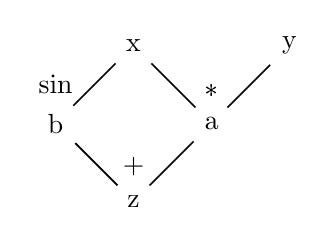
\begin{tikzpicture}[
            shorten > = 1pt, % don't touch arrow head to node
            auto,
            node distance = 1.4cm, % distance between nodes
            semithick % line style
        ]

        \node[label=\lstinline!+!] (z) {\lstinline!z!};
        \node[label=\lstinline!sin!] (b) [above left of=z] {\lstinline!b!};
        \node[label=\lstinline!*!] (a) [above right of=z] {\lstinline!a!};
        \node[] (x) [above right of=b] {\lstinline!x!};
        \node[] (y) [above right of=a] {\lstinline!y!};

        \path[-] (z) edge node {} (a);
        \path[-] (z) edge node {} (b);
        \path[-] (b) edge node {} (x);
        \path[-] (a) edge node {} (y);
        \path[-] (a) edge node {} (x);
\end{tikzpicture}

\column{.65\textwidth}

\begin{onlyenv}<2->
The ``roots'' of the graph are the independent variables \lstinline!x! and \lstinline!y!. Constructing these nodes is as simple as creating an object:

\begin{lstlisting}[language=python]
class Var:
  def __init__(self, value):
    self.value = value
    self.children = []
    ...
  ...

x = Var(0.5)
y = Var(4.2)
\end{lstlisting}
\end{onlyenv}

\uncover<3->{Each \lstinline!Var! node can have \emph{children} which are the nodes that depend directly on that node. The children allow nodes to link together in a \textbf{Directed Acyclic Graph}.}

\end{columns}

\end{frame}

\begin{frame}[fragile]
	\frametitle{Building expressions}

By default, nodes do not have any children. As expressions are created each expression $u$ registers itself as a child of each of its dependencies $w_i$ together with its weight $\partial w_i/\partial u$ which will be used to compute gradients:

\begin{lstlisting}[language=python]
class Var:
  ...
  def __mul__(self, other):
    z = Var(self.value * other.value)

    # weight = dz/dself = other.value
    self.children.append((other.value, z))

    # weight = dz/dother = self.value
    other.children.append((self.value, z))
    return z
  ...
...
# "a" is a new Var that is a child of both x and y
a = x * y
\end{lstlisting}
\end{frame}

\begin{frame}[fragile]
\frametitle{Computing gradients}

Finally, to get the gradients we need to propagate the derivatives. To avoid unnecessarily traversing the tree multiple times we will \emph{cache} the derivative of a node in an attribute \lstinline!grad_value!:
\begin{lstlisting}[language=python,basicstyle=\footnotesize\ttfamily]
class Var:
  def __init__(self):
    ...
    self.grad_value = None

  def grad(self):
    if self.grad_value is None:
      # calculate derivative using chain rule
      self.grad_value = sum(weight * var.grad() for weight, var in self.children)
    return self.grad_value
	...
...
a.grad_value = 1.0
print("da/dx = {}".format(x.grad()))
\end{lstlisting}
\end{frame}

% \begin{frame}
% \frametitle{Reverse Mode AD}
% \begin{block}{Let's try this for ourselves\ldots}
% \begin{itemize}
% 	\item Launch \lstinline!jupyter notebook! and load the \lstinline!ReverseAD.ipynb! notebook.
% 	\item Work through the exercises.
% \end{itemize}
% \end{block}
% \end{frame}

\begin{frame}
\frametitle{Aside: Optimising Reverse Mode AD}
\begin{itemize}
	\item<+-> The Reverse AD approach we've outlined is not very space efficient. One way to get around this is to avoid storing the children directly and instead store indices in an auxiliary data structure called a \emph{Wengert list} or \emph{tape}.
	\item<+-> Another interesting approach to memory reduction is trade-off computation for memory of the caches. The Count-Trailing-Zeros (CTZ) approach does just this\footnote{Andreas Griewank (1992) Achieving logarithmic growth of temporal and spatial complexity in reverse automatic differentiation, Optimization Methods and Software, 1:1, 35-54, DOI: 10.1080/10556789208805505}.
	\item<+-> \textbf{But,} in reality memory is relatively cheap if managed well...
\end{itemize}
\end{frame}

\begin{frame}
\frametitle{AD in the PyTorch autograd package}

\begin{itemize}
	\item<+-> PyTorch's AD is remarkably similar to the one we've just built: \begin{itemize}
		\item<+-> it eschews the use of a tape
		\item<+-> it builds the computation graph as it runs (recording explicit \lstinline!Function! objects as the children of \lstinline!Tensors! rather than grouping everything into \lstinline!Var! objects)
		\item<+-> it caches the gradients in the same way we do (in the \lstinline!grad! attribute) - hence the need to call \lstinline!zero_grad()! when recomputing the gradients of the same graph after a round of backprop.
	\end{itemize}
	\item<+-> PyTorch does some clever memory management to work well in a reference-counted regime and aggressively frees values that are no longer needed.
	\item<+-> The backend is actually mostly written in C++, so its fast, and can be multi-threaded (avoids problems of the GIL).
	\item<+-> It allows easy ``turning off'' of gradient computations through \lstinline!requires_grad!.
	\item<+-> In-place operations which invalidate data needed to compute derivatives will cause runtime errors, as will variable aliasing...
\end{itemize}
\end{frame}


% \begin{frame}
% \frametitle{Reverse Mode AD}
% \begin{block}{Let's try this for ourselves\ldots}
% \begin{itemize}
% 	\item Launch \lstinline!jupyter notebook! and load the \lstinline!PyTorchAD.ipynb! notebook.
% 	\item Work through the exercises.
% \end{itemize}
% \end{block}
% \end{frame}

\end{document}